\documentclass[a4paper, 12pt]{article}
\usepackage[a4paper,top=1.5cm, bottom=1.5cm, left=1cm, right=1cm]{geometry}
\usepackage{cmap}					
\usepackage{mathtext} 				
\usepackage[T2A]{fontenc}			
\usepackage[utf8]{inputenc}			
\usepackage[english,russian]{babel}
\usepackage{multirow}
\usepackage{graphicx}
\usepackage{wrapfig}
\usepackage{tabularx}
\usepackage{float}
\usepackage{longtable}
\usepackage{hyperref}
\hypersetup{colorlinks=true,urlcolor=blue}
\usepackage[rgb]{xcolor}
\usepackage{amsmath,amsfonts,amssymb,amsthm,mathtools} 
\usepackage{icomma} 
\usepackage{euscript}
\usepackage{mathrsfs}
\usepackage{enumerate}
\usepackage{caption}
\usepackage{enumerate}
\mathtoolsset{showonlyrefs=true}
\usepackage{graphicx}
\usepackage{caption}
\usepackage{subcaption}
\usepackage[europeanresistors, americaninductors]{circuitikz}
\DeclareMathOperator{\sgn}{\mathop{sgn}}
\newcommand*{\hm}[1]{#1\nobreak\discretionary{}
	{\hbox{$\mathsurround=0pt #1$}}{}}

\title{\textbf{Определение ускорения свободного падения \newline
(1.4.2 и 1.1.8)}}
\author{Манро Эйден}
\date{}

\begin{document}

\maketitle

\begin{center}
    \section*{Введение}
\end{center}

\noindent \textbf{Цель работы:} определить ускорение свободного падения посредством прямых измерений ускорения падающего тела и с помощью оборотного маятника.

\bigskip

\noindent \textbf{Оборудование:} вертикальная труба с намотанными катушками, шарообразные 
неодимовые магниты, линейка, блок регистрации сигнала, соединённый с цифровым осциллографом, оборотный маятник с двумя подвесными призмами и двумя грузами, электронный счётчик времени и числа колебаний,
подставка с острием для определения положения центра масс маятника, закреплённая на стене консоль для подвешивания маятника, металлические линейки, штангенциркуль длиной 1 м.

\bigskip

\begin{center}
        \subsection*{Теоретические сведения}
        Физическим маятником называют твёрдое тело, способное совершать 
колебания в вертикальной плоскости, будучи подвешено за одну из своих 
точек в поле тяжести. Ось, проходящая через точку подвес перпендикулярно плоскости качания, называется осью качания маятника.

При малых колебаниях период колебаний физического маятника определяется формулой
\begin{equation}
  T = 2\pi \sqrt{\frac{J}{mgl}}
  \label{period}
\end{equation}
где $J$ — момент инерции маятника относительно оси качания, $m$ — масса 
маятника, $l$ — расстояние от оси качания до центра масс маятника.
Если сравнить \eqref{period} с известной формулой колебаний математического 
маятника длиной $l$ ($T = 2\pi\sqrt{l/g}$), можно определить приведённую длину физического маятника как \eqref{privedmass}:

\begin{equation}
    l_{\text{пр}} = \frac{J}{ml}
    \label{privedmass}
\end{equation}

\end{center}
\begin{center}
    
\subsubsection*{Теорема Гюйгенса об оборотном маятнике}
\end{center}



Пусть $O_{1}$ — точка подвеса физического маятника, а 
$C$ — его центр масс. Отложим отрезок длиной $l_{\text{пр}}$ вдоль линии $O_{1}C$, и обозначим соответствующую точку как $O_{2}$ — эту точку называют \textit{центром качания} физического маятника. Заметим, что приведённая длина всегда 
больше расстояния до центра масс ($l_{\text{пр}} > l$), поэтому 
точка $O_{2}$ лежит по другую сторону от центра масс.

Точки $O_{1}$ и $O_{2}$ обладают свойством \textit{взаимности}: 
если перевернуть маятник и подвесить его за точку $O_{2}$, 
то его период малых колебаний останется таким же, как 
и при подвешивании за точку $O_{1}$ (\textit{теорема Гюйгенса}). 
На этом свойстве — «оборотности» — и основан довольно точный метод определения ускорения свободного падения, применяемый в данной работе.

\begin{figure}[H]
\centering
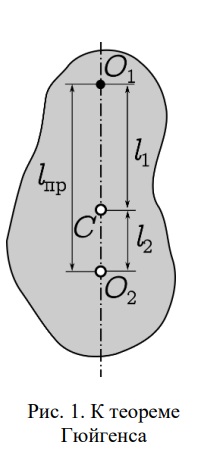
\includegraphics[width=.21\textwidth]{image_1.png}
\end{figure}

\begin{center}
    
\subsubsection*{Измерение $g$ посредством прямых измерений ускорения падающего тела}
Рассмотрим падение шарика из его начального положения, когда он удерживается электромагнитом. Направим ось у вертикально вниз, а начало отсчёта $y = 0$ совместим с положением самой верхней катушки.
Пусть $V_{0}$ – скорость шарика в центре самой верхней катушки. Для равноускоренного движения шарика справедливо выражение:
$$y = v_{0}t + \frac{gt^2}{2}$$

Выражение можно записать для пяти моментов времени $t_{n}$ ($n = 1, 2, 3, 4, 5$), 
соответствующих пролёту шарика через соответствующую катушку:
$$nl = v_{0}t_{n} + \frac{gt_{n}^2}{2}$$

Перепишем выражение в виде
$$\frac{nl}{t_{n}} = v_{0} + \frac{gt_{n}}{2}$$
Проводя измерения времён $t_{n}$ при свободном падении шарика и используя выражение, можно построить график зависимости величины $nl/t_{n}$ от $t_{n}$ и 
определить ускорение свободного падения из углового коэффициента данной
зависимости.

\end{center}

\bigskip

\begin{center}
    
\subsubsection*{Измерение $g$ с помощью физического маятника} 

Пусть L = $l_{1} + l_{2}$ — расстояние между двумя «сопряжёнными» точками подвеса физического маятника. Если соответствующие периоды малых колебаний равны, $T_{1} = T_{2} = T$, то по теореме Гюйгенса $L = l_{\text{пр}}$. Тогда находим ускорение свободного падения:
$$g_{0} = (2\pi)^2\frac{L}{T^2}.$$

Точного совпадения $T_{1} = T_{2}$ на опыте добиться, конечно, невозможно. 
Поэтому получим формулу для определения ускорения свободного падения $g$, если измеренные периоды незначительно различаются: $T_{1} = T, T_{2} =
T + \varDelta T$. Получаем:
$$g = (2\pi)^2\frac{l_{1}^2-l_{2}^2}{T_{1}^2l_{1} - T_{2}^2l_{2}}$$

\end{center}

\begin{center}
    
\subsection*{Экспериментальная установка}
\bigskip
\subsubsection*{Устройство установки из опыта 1.1.8}
\bigskip
Металлический шарик (неодимовый магнит) первоначально удерживается сверху электромагнитом в подвешенном состоянии. После выключения тока, текущего через 
электромагнит, шарик начинает падать вниз и пролетает последовательно через 
шесть тонких проволочных катушек. С катушками соединены датчики электрического напряжения и регистраторы времени (таймеры). Шарик имеет собственную намагниченность (является постоянным магнитом), поэтому, когда он пролетает сквозь проволочную катушку, он своим магнитным полем наводит в катушке индукционный ток. Этот ток регистрируется 
электрическим датчиком, соединённым с катушкой. По возникающему импульсу напряжения срабатывает таймер, соединённый с данной катушкой. 
Все датчики подключены к блоку управления и 
регистрации. Начало отсчёта времени $t = 0$ соответствует пролёту шариком самой верхней катушки. Каждый из таймеров регистрирует время 
пролёта шариком соответствующей катушки. Расстояние между соседними катушками одинаково и 
равно $l \approx 40$ см (точные значения указаны на установке или могут быть измерены непосредственно). 
На таком же расстоянии находится шарик в подвешенном состоянии над верхней катушкой. 
После пролёта всех катушек шарик попадает в металлическую трубку, в которой он тормозится перед падением на пол (электромагнитное торможение). Механизм торможения заключается в том, 
что так же, как и в катушках, в металлической трубке наводятся индукционные токи (токи Фуко), которые, в соответствии с правилом Ленца, своим магнитным полем тормозят движение шарика. Заметим, что шарик будет неизбежно испытывать некоторое торможение и при пролёте каждой катушки. Однако этот эффект можно свести к минимуму, если сопротивление цепи катушки достаточно велико, и, следовательно, возникающие токи, а значит и силы, малы.

\begin{figure}[H]
    \centering
    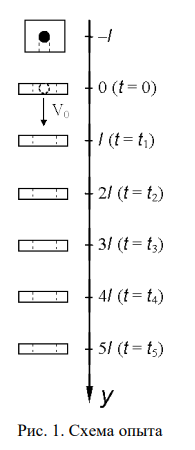
\includegraphics[width=0.25\linewidth]{image_3.png}
\end{figure}
\begin{figure}[H]
    \centering
    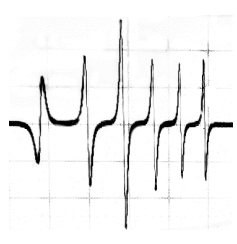
\includegraphics[width=0.25\linewidth]{image_4.png}
    \caption{Характерная осицллограмма}
\end{figure}

Импульсы тока от всех катушек также регистрируются на экране запоминающего осциллографа. По картине импульсов на экране осциллографа можно примерно определить 
время пролёта шариком каждой из катушек и 
сравнить это время с соответствующим значением таймера. Согласно закону электромагнитной индукции напряжение в цепи регистрации пропорционально производной магнитного потока от шарика через регистрирующую катушку. Поэтому, когда шарик будет находится в центре 
регистрирующей катушки, поток магнитного поля через неё будет максимален, 
что будет соответствовать нулю регистрируемого сигнала.\\
\bigskip
\subsubsection*{Устройство маятника}
\bigskip
Применяемые в работе маятники представляет собой стержни цилиндрического или прямоугольного сечения длиной 1 м и массой 1 ÷ 1,5 кг. Маятник подвешивается с помощью небольших треугольных призм (П1 и П2), острым основанием опирающихся на закреплённую на стене консоль. Ребро призмы задаёт ось качания маятника. На стержне закрепляются два дополнительных груза в форме «чечевицы» (Г1 и Г2). Для выполнения условия $l_{1} > l_{2}$ внешнюю чечевицу Г2 следует крепить за призмой П2, а чечевицу Г1 (внутреннюю) — между призмами П1 и П2 (см. Рис. 3).

\begin{figure}[H]
    \centering
    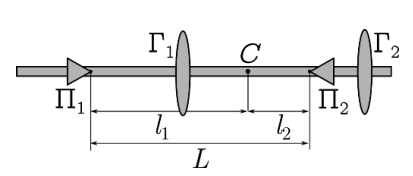
\includegraphics[width=0.5\linewidth]{image_2.png}
    \caption{Маятник с грузами}
\end{figure}

Регистрация времени колебаний проводится с помощью электронных 
счётчиков. Расстояния между точками установки маятников на консоли до электронных счётчиков фиксировано. Это накладывает ограничения на расположение призм и грузов на стержне. Призмы крепятся симметрично на равном расстоянии от концов стержней так, чтобы маятник при колебаниях пересекал фотоприёмники счётчика, не задевая оправу счётчика.

Фиксированное положение призм однозначно задаёт приведённую 
длину оборотного маятника $l_{\text{пр}} = L$. Изменять в опыте можно только положения грузов на стрежне. Главная задача опыта — подобрать такое положение грузов, при котором периоды колебаний при перевороте маятника совпадали бы с достаточно высокой точностью, а для положения центра масс маятника выполнялось при этом условие $l_{1} > 2.5 l_{2}$\\

\subsubsection*{Оценка погрешностей}

\bigskip

Оценим влияние погрешностей измерений на точность расчётов. Пусть все периоды измерены с одинаковой погрешностью $\sigma_{T}$, расстояние $L$ между точками подвеса с погрешностью $\sigma{L}$, расстояния $l_{1,2}$ до центра масс с погрешностью $\sigma_{1}$. Погрешность определения величины $g_{0}$ равна:
$$\frac{\sigma_{g_{0}}}{g_{0}} = \sqrt{(\frac{\sigma_{L}}{L})^2 + 4\frac{\sigma_{T}}{T})^2}$$

Это — основная погрешность опыта. Видно, что для её минимизации необходимо максимально точно измерить расстояние между точками повеса $L$ и период колебаний маятника $T$

Для полной относительной погрешности получим
$$\frac{\sigma{g}}{g} \approx \sqrt{(\frac{\sigma_{L}}{L})^2 + 4(\frac{\sigma_{T}}{T})^2 + 8(\beta\frac{\sigma_{T}}{T})^2 + 8(\beta\frac{\varDelta T}{T}\frac{\sigma_{l}}{\varDelta l})^2}$$

Из этого результата можно сделать следующие выводы. Во-первых, при 
достаточно хорошем совпадении периодов ($\varDelta T \ll T$) погрешность измерения длин $l_{1}$ и $l_{2}$ по отдельности практически не влияет на погрешность конечного результата, поскольку вклад последнего (4-го) слагаемого будет заведомо мал. И, во-вторых, итоговая погрешность неограниченно возрастает при $l_{1} → l_{2}$, т. е., когда центр масс маятника оказывается близок к геометрическому центру стержня.

\end{center}

\begin{center}
    
\section*{Ход работы}
\subsection*{Определение ускорения свободного падения с помощью прямых измерений ускорения падающего тела}
\bigskip
Измерим расстояние $l$ между соседними катушками. $l = (38.7 \pm 0.1)$ см

Положим шарик в пластиковый держатель, закреплённый на длинной металлической штанге, и поднесем его к установленному в верхней точке установки электромагниту так, чтобы он зафиксировался в нём. После нажатия кнопки «Сброс» на блоке управления произошло размыкание электрической цепи электромагнита, и шарик свободно упал вниз. На цифровом индикаторе отобразились времена пролёта магнита через катушки. Повторим опыт с падением 7 раз и запишем все полученные значения времён $t_{n}$

\begin{table}[H]
    \centering
    \begin{tabular}{|l|l|l|l|l|l|l|l|} \hline
        $t_{n}, \text{дс}$ & №1 & №2 & №3 & №4 & №5 & №6 & №7 \\ \hline
        $t_{1}, \text{дс}$ & 1.1766 & 1.1828 & 1.1437 & 1.1878 & 1.1896 & 1.1877 & 1.1842 \\ \hline
        $t_{2}, \text{дс}$ & 2.0711 & 2.0731 & 2.0821 & 2.0788 & 2.0847 & 2.0736 & 2.0739 \\ \hline
        $t_{3}, \text{дс}$ & 2.8317 & 2.8308 & 2.8359 & 2.8399 & 2.8470 & 2.8312 & 2.8319 \\ \hline
        $t_{4}, \text{дс}$ & 3.5017 & 3.4995 & 3.5044 & 3.5118 & 3.5193 & 3.5005 & 3.5011 \\ \hline
        $t_{5}, \text{дс}$ & 4.1030 & 4.1027 & 4.1111 & 4.1175 & 4.1243 & 4.1053 & 4.1052 \\ \hline
        $g, \frac{\text{м}}{\text{с}^2}$ & 9.8618 & 9.7178 & 9.9304 & 9.8632 & 9.7658 & 9.0502 & 9.7970\\ \hline
    \end{tabular}
    \caption{Измерения времен пролёта магнита через катушки}
\end{table}

\begin{figure}[H]
    \centering
    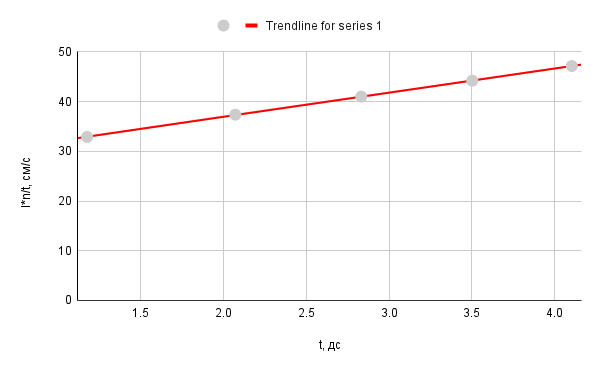
\includegraphics[width=0.5\linewidth]{image_0.png}
\end{figure}

Получили $g = 9.7100 \space \frac{\text{м}}{\text{c}^2}$\\

\subsection*{Определение ускорения свободного падения с помощью физического маятника}
Взвесим мятник и все его элементы по отдельности
\begin{table}[H]
    \centering
    \begin{tabular}{|l|l|} \hline
        & Масса, г  \\ \hline
        Стержень & $890.8 \pm 0.1$ \\ \hline
        Призма №1 & $77.2 \pm 0.1$ \\ \hline
        Призма №2 & $78.4 \pm 0.1$ \\ \hline
        Груз №1 & $376.6 \pm 0.1$ \\ \hline
        Груз №2 & $367.1 \pm 0.1$ \\ \hline
        Маятник & $1789.9 \pm 0.1$ \\ \hline
    \end{tabular}
    \caption{Измерения масс элементов маятника}

\end{table}

С помощью большого штангенциркуля измерим расстояние $L$ между призмами.

Длина стрежня $L_{\text{ст}} = (100.07 \pm 0.01)$ см

Расстояние между призмами $L = (52.37 \pm 0.01)$ см\\

Зададим отношение $l_{1}/l_{2} = 1.5$. Получим положение грузов $l_{1} = 31.47$ см, $l_{2} = 20.90$ см.

С помощью T-образной подставки определим положение центра масс маятника с грузами.

Проведем измерение времени n = 20 колебаний 4 раза, отклоняя маятник на малый угол $\alpha \approx 5^{\circ}$
 
\begin{table}[H]
    \centering
    \begin{tabular}{|l|l|l|} \hline
        № & Время, c & Период, c  \\ \hline
        1 & 29.12 & 1.45  \\ \hline
        2 & 29.14 & 1.45  \\ \hline
        3 & 29.13 & 1.45  \\ \hline
        4 & 29.14 & 1.45  \\ \hline
    \end{tabular}
    \caption{Измерения периода колбаний $T_{2}$}
    
\end{table}

Перевернем маятник. Проведем измерения периода $T_{1}$

\begin{table}[H]
    \centering
    \begin{tabular}{|l|l|l|} \hline
        № & Время, c & Период, c  \\ \hline
        1 & 29.11 & 1.46  \\ \hline
        2 & 29.11 & 1.46  \\ \hline
        3 & 29.11 & 1.46  \\ \hline
        4 & 29.12 & 1.45  \\ \hline
    \end{tabular}
    \caption{Измерения периода колбаний $T_{1}$}
\end{table}

Сравним значения $T_{1}$ и $T_{2}$: $\frac{\varDelta T}{T} = 1 - \frac{1.45}{1.46} \approx 0.69\%$\\

\bigskip

Найдем значение $g_{0}$: $g_{0} = (2\pi)^2\frac{l_{1}^2-l_{2}^2}{T_{1}^2l_{1} - T_{2}^2l_{2}} \approx 9.79 \frac{\text{м}}{\text{c}^2}$\\

\bigskip

Найдем погрешность $\varDelta g \approx \frac{2l_{2}}{l_{1}-l_{2}} \frac{\varDelta T}{T} g_{0} \approx 0.01 \frac{\text{м}}{\text{c}^2}$\\

\bigskip

Тогда $g = g_{0} + \varDelta g = 9.79 \pm 0.01 \frac{\text{м}}{\text{c}^2}$
\end{center}

\begin{center}
    
\section*{Выводы}
В ходе работы определил $g$ двумя способами: с помощью прямых измерений и с помощью оборотного маятника. В первом случае получил $g_{1} = 9.71 \frac{\text{м}}{\text{c}^2}$, относительная погрешность $\epsilon_{1} = 1\%$ по сравнению с ускорением свободного падения в Москвовской Области $g_{0} = 9.81 \frac{\text{м}}{\text{c}^2}$, а абсолютная погрешность $\varDelta g_{1} = 0.01\frac{\text{м}}{\text{c}^2}$.
Во втором случае получил $g_{2} = 9.79 \frac{\text{м}}{\text{c}^2}$, относительная погрешность $\epsilon_{2} = 4\%$, а абсолютная погрешность $\varDelta g_{2} = 0.04$ м$/c^2$

\end{center}

\end{document}

